\documentclass[11pt]{article}

% ===== Packages =====
\usepackage[utf8]{inputenc}
\usepackage[T1]{fontenc}
\usepackage{lmodern}
\usepackage[margin=1in]{geometry}
\usepackage{amsmath,amssymb,amsfonts}
\usepackage{graphicx}
\usepackage{booktabs}
\usepackage{hyperref}
\usepackage{cleveref}
\usepackage{xcolor}
\usepackage{enumitem}
\usepackage{float}
\usepackage{caption}
\usepackage{listings}
\usepackage{url}
\usepackage{natbib}
\usepackage{microtype}

\hypersetup{
  colorlinks=true,
  linkcolor=blue!70!black,
  citecolor=blue!70!black,
  urlcolor=blue!70!black
}

\lstset{
  basicstyle=\ttfamily\small,
  frame=single,
  breaklines=true,
  columns=fullflexible
}

% ===== Title =====
\title{AI in the Loop (AITL): A Systems Taxonomy for\\Closed-Loop Autonomous Evaluation}

\author{
  Sanskar Jajoo\\
  Independent Researcher, India\\
  \url{https://github.com/m4vic}
}

\date{}

\begin{document}

\maketitle

% ===== Abstract =====
\begin{abstract}
We identify and formalize AI In The Loop (AITL), a paradigm where AI systems autonomously generate, evaluate, and improve with human intervention restricted to boundary supervision rather than operational decision-making. AITL extends the RLAIF principle---replacing human feedback with AI feedback---from training to the full AI system lifecycle. This is a framework paper with proof-of-concept validation; we propose a unifying taxonomy rather than a benchmark study.

Through analysis of four systems (AlphaZero, Constitutional AI, SWE-agent, autoresearch), we extract common properties and propose a unifying taxonomy: self-generation, self-evaluation, self-improvement, and human observation. We validate AITL through a controlled experiment using the Autonomous Empirical Optimization System (AEOS), a model-agnostic ML sandbox where two LLM agents autonomously built ML pipelines on a semantically-stripped dataset. In our experiment, we observe that the dominant human role in AITL shifts from iterative ML engineering ($O(n)$ per iteration) to boundary supervision ($O(1)$ per experiment).

Our contributions are: (1)~formalization of AITL as a unifying framework for closed-loop autonomous systems, (2)~a taxonomy connecting existing systems under shared properties, (3)~empirical validation via AEOS demonstrating autonomous agent stopping behavior, and (4)~identification of failure modes including a novel Sunk-Cost Continuation failure mode (F6), where agents continue low-yield exploration despite prolonged stagnation. We position AITL as a natural evolution of AI evaluation, suggesting scalable directions infeasible under HITL constraints.
\end{abstract}

\noindent\textbf{Keywords:} AI evaluation, closed-loop systems, autonomous ML, neural architecture search, self-improving AI

% ===================================================================
\section{Introduction}
\label{sec:intro}

\subsection{The Human Bottleneck}

AI systems increasingly require continuous evaluation: safety testing for each model version, adversarial robustness across attack families, regression detection over time, and cross-model comparison.

Traditional Human-in-the-Loop (HITL) evaluation creates bottlenecks:
\begin{itemize}[nosep]
  \item Expert reviewers cost \$200--500/hour
  \item Manual testing limits coverage
  \item Human fatigue reduces consistency
  \item Doesn't scale to continuous deployment
\end{itemize}

For example, GPT-4 red-teaming required 50+ external experts over 6 months \citep{openai2023gpt4}. Each model update requires repeating this expensive process.

\subsection{The Pattern We Propose to Unify}

Several major AI systems have independently solved this problem by removing humans from operational loops:

\textbf{AlphaZero} (2017): Game evaluation via self-play. No human game records needed---AI generates positions, evaluates outcomes, and improves policy, achieving superhuman performance \citep{silver2017mastering}.

\textbf{Constitutional AI} (2022): Alignment via RLAIF. AI judges AI outputs against principles with minimal human feedback, enabling scalable alignment \citep{bai2022constitutional}.

\textbf{autoresearch} (Karpathy, repository accessed 2026): Autonomous ML experimentation. AI modifies code, runs experiments, and evaluates results while humans review only the final output \citep{karpathy2026autoresearch}.

We propose a unifying interpretation of these systems under a common operational framework: \textbf{AI In The Loop (AITL)}.

\subsection{Contributions}

We formalize AI In The Loop (AITL) and provide:

\begin{enumerate}[nosep]
  \item \textbf{Paradigm Definition}: Clear properties distinguishing AITL from HITL, with formal requirements.
  \item \textbf{Taxonomy of Existing Systems}: Analysis of AlphaZero, Constitutional AI, SWE-agent, and autoresearch as systems exhibiting AITL-like properties.
  \item \textbf{Experimental Validation}: A reproducible proof-of-concept demonstrating the self-improving feedback loop.
  \item \textbf{Failure Mode Analysis}: Identification of when and how AITL systems fail.
  \item \textbf{Roadmap}: Open challenges and future research directions.
\end{enumerate}

\subsection{Scope and Novelty}

We note explicitly: the contribution of this work is \emph{not} the invention of closed-loop AI systems---these have existed for decades. Our contribution lies in:

\begin{itemize}[nosep]
  \item Identifying a common set of operational properties across independently developed systems
  \item Formalizing these properties into a reusable taxonomy
  \item Providing empirical evidence via a controlled experiment
  \item Defining failure modes and requirements for safe deployment
\end{itemize}

\subsection{Paper Organization}

\Cref{sec:background} provides background on HITL and the RLHF$\to$RLAIF evolution. \Cref{sec:existing} analyzes existing AITL-like systems. \Cref{sec:formal} presents the formal AITL definition and properties. \Cref{sec:casestudy} examines autoresearch as an external case study. \Cref{sec:aeos} describes our controlled experimental validation via AEOS. \Cref{sec:future} discusses future applications and limitations. \Cref{sec:conclusion} concludes.

% ===================================================================
\section{Background}
\label{sec:background}

\subsection{Human-in-the-Loop (HITL) Evaluation}

HITL has been the standard for AI system validation. Humans occupy critical decision points in operational workflows, reviewing AI outputs before deployment.

\textbf{Examples:} Content moderation (humans review flagged posts), medical AI (doctors verify diagnoses), autonomous vehicles (safety drivers monitor systems), and model evaluation (red-teamers test for failures).

\textbf{Advantages:}
\begin{itemize}[nosep]
  \item Human judgment on edge cases
  \item Accountability (human made final decision)
  \item Regulatory compliance in high-stakes domains
\end{itemize}

\textbf{Limitations:}
\begin{itemize}[nosep]
  \item Linear scaling with workload (more tests = more humans)
  \item Inconsistency (fatigue, subjectivity, drift over time)
  \item Cost (expert time is expensive, scarce)
  \item Latency (human review is slow)
\end{itemize}

\subsection{From RLHF to RLAIF: Training's Evolution}

Reinforcement Learning from Human Feedback (RLHF) dominated LLM alignment \citep{christiano2017deep,ouyang2022training}:
\begin{enumerate}[nosep]
  \item Generate model outputs
  \item Humans rank outputs ($A$ better than $B$)
  \item Train reward model on rankings
  \item Optimize policy via RL
\end{enumerate}

\textbf{Bottleneck:} Requires 50K--500K human labels.

\citet{bai2022constitutional} introduced Constitutional AI, using Reinforcement Learning from AI Feedback (RLAIF):
\begin{enumerate}[nosep]
  \item Define constitutional principles (human-provided)
  \item AI critiques outputs against principles
  \item AI ranks critiques
  \item Train from AI feedback
\end{enumerate}

\textbf{Result:} 90\% reduction in human labeling, comparable alignment quality. \textbf{Key insight:} AI can judge AI when given a proper framework.

\subsection{The Missing Piece: HITL Evaluation Remains}

While RLAIF solved training bottlenecks, evaluation workflows still rely on HITL. \emph{Can we apply RLAIF's lesson to evaluation?} Our results suggest: yes, via AITL.

\Cref{fig:evolution} illustrates this evolution from manual per-instance evaluation (HITL) through training-phase automation (RLHF, RLAIF) to operational-phase automation (AITL), and positions existing systems as bounded instantiations of the AITL paradigm.

\begin{figure}[H]
  \centering
  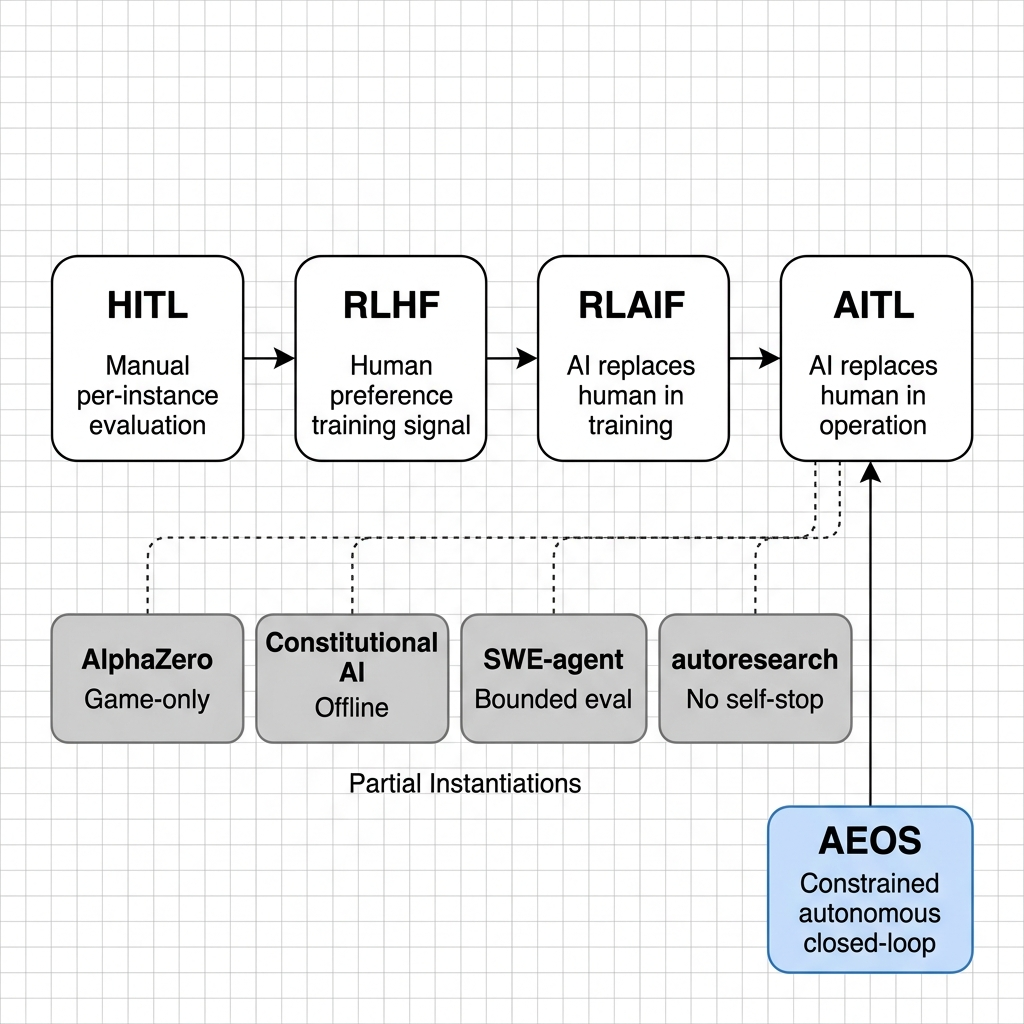
\includegraphics[width=0.95\textwidth]{figures/aitl_evolution_diagram.png}
  \caption{Evolution of AI evaluation paradigms: from Human-in-the-Loop (HITL) through RLHF and RLAIF to AI-in-the-Loop (AITL). Existing systems represent bounded instantiations; AEOS is our constrained autonomous closed-loop instance.}
  \label{fig:evolution}
\end{figure}

\subsection{Related Paradigms}

AITL intersects with, but differs from, several existing concepts:

\textbf{AutoML / NAS.} Systems like Auto-sklearn \citep{feurer2015efficient}, TPOT \citep{olson2016evaluation}, DARTS \citep{liu2019darts}, and ENAS \citep{pham2018efficient} focus on architecture or hyperparameter search. AITL is broader: any autonomous generate-evaluate-improve loop, not limited to model selection.

\textbf{Active Learning.} Humans selectively label the most informative examples \citep{settles2009active}. AITL removes humans from the labeling loop entirely---the evaluator is itself an AI component.

\textbf{Self-Play.} AlphaZero \citep{silver2017mastering} and related systems use self-play in adversarial game settings. AITL generalizes beyond zero-sum games to any evaluation domain.

\textbf{Meta-Learning.} MAML \citep{finn2017model} and related approaches learn how to learn across task distributions. AITL learns what works via feedback on a specific task instance.

\textbf{LLM Agents.} Systems like AutoGPT \citep{richards2023autogpt} and BabyAGI \citep{nakajima2023babyagi} use LLMs for autonomous task execution. These represent instances of AITL when they incorporate evaluation feedback loops, though many lack the self-improving property (P3).

We propose AITL as a unifying framework that encompasses these as special cases, distinguished by the four properties defined in \Cref{sec:formal}.

% ===================================================================
\section{Existing AITL-Like Systems}
\label{sec:existing}

We analyze foundational systems that independently exhibit AITL properties, acting as precursors to the paradigm. However, we note that none of these constitute fully autonomous closed-loop instances under our stricter definition (\Cref{sec:formal}), as each is restricted in domain scope, evaluation dynamics, or termination autonomy.

\subsection{AlphaZero: Closed-Loop Game Mastery (2017)}

AlphaZero \citep{silver2017mastering} exhibits strong AITL-like closed-loop properties:
\begin{itemize}[nosep]
  \item \emph{Self-Generating}: Generates game positions through self-play
  \item \emph{Self-Evaluating}: MCTS search evaluates position quality
  \item \emph{Self-Improving}: Policy network updated from game outcomes
  \item \emph{Human-Observed}: Researchers monitor Elo ratings
\end{itemize}

\textbf{Bounded instantiation:} AlphaZero is narrowly scoped to deterministic, perfect-information, zero-sum games where the evaluation function (win/loss) is mathematically guaranteed. It cannot function in open-ended operational environments where evaluation criteria are abstract or ambiguous.

\subsection{Constitutional AI: Closed-Loop Alignment (2022)}

\citet{bai2022constitutional} demonstrated AITL properties for language alignment:
\begin{itemize}[nosep]
  \item \emph{Self-Generating}: AI generates response critiques
  \item \emph{Self-Evaluating}: AI judges outputs against constitutional principles
  \item \emph{Self-Improving}: RLAIF training updates model behavior
  \item \emph{Human-Observed}: Humans define principles, review aggregate metrics
\end{itemize}

\textbf{Bounded instantiation:} Constitutional AI applies the AITL philosophy exclusively to the \emph{offline pre-training and fine-tuning} phase. It is not a real-time operational agent capable of independent exploration or dynamic constraint management.

The system achieved comparable alignment quality to RLHF with 90\% fewer human annotations, suggesting that AI judgment can substitute for human judgment when given appropriate constraints.

\subsection{autoresearch: Closed-Loop ML Experimentation (2026)}

A public repository released by Andrej Karpathy documents autonomous experimentation loops under the name autoresearch \citep{karpathy2026autoresearch}:
\begin{itemize}[nosep]
  \item \emph{Self-Generating}: Agent modifies \texttt{train.py} with new hyperparameters, architectures, and optimization strategies
  \item \emph{Self-Evaluating}: Validation bits-per-byte (\texttt{val\_bpb}) provides objective scoring after each 5-minute training run
  \item \emph{Self-Improving}: Agent uses git-integrated history of successes and failures to inform subsequent experiments
  \item \emph{Human-Observed}: Researcher defines goals in \texttt{program.md}, reviews final committed improvements
\end{itemize}

When pointed at nanochat (a well-tuned GPT-2 training codebase), the agent ran approximately 700 experiments over two days, identifying multiple improvements missed by human developers. These changes reduced time-to-GPT-2 from 2.02 to 1.80 hours---an 11\% improvement on an already heavily optimized baseline.

\subsection{SWE-agent: Closed-Loop Software Engineering (2024)}

\citet{jimenez2024swebench} introduced SWE-bench and the accompanying SWE-agent---an LLM agent that autonomously resolves real GitHub issues:
\begin{itemize}[nosep]
  \item \emph{Self-Generating}: Agent writes code patches and unit test commands autonomously, exploring the codebase without human guidance
  \item \emph{Self-Evaluating}: Existing unit test suites provide an objective pass/fail signal after each patch attempt
  \item \emph{Self-Improving}: The agent integrates test failure messages into subsequent patch attempts, iterating toward a passing state
  \item \emph{Human-Observed}: Humans define the benchmark; the agent resolves issues independently
\end{itemize}

\textbf{Bounded instantiation:} SWE-agent's evaluation signal comes from a pre-written human test suite. The agent cannot author \emph{new} tests to verify its own solutions against uncovered corner cases. Self-evaluation is therefore bounded by the quality of the human-authored harness.

\subsection{Cross-System Comparison}

\begin{table}[t]
  \centering
  \caption{Cross-system comparison of AITL properties across four foundational systems. All exhibit core AITL properties but with distinct autonomy bounds.}
  \label{tab:comparison}
  \small
  \begin{tabular}{@{}lllll@{}}
    \toprule
    \textbf{Property} & \textbf{AlphaZero} & \textbf{Constitutional AI} & \textbf{autoresearch} & \textbf{SWE-agent} \\
    \midrule
    Self-Gen & Game positions & Response critiques & Code modifications & Code patches \\
    Self-Eval & MCTS value & Constitutional judgment & \texttt{val\_bpb} metric & Unit test pass/fail \\
    Self-Improve & Policy update & RLAIF training & Git commit/revert & Iterative patch \\
    Human Role & Monitor Elo & Define principles & Set goals & Define test suite \\
    Autonomy bound & Game-only & Offline phase & No self-stop & Human test harness \\
    \bottomrule
  \end{tabular}
\end{table}

\Cref{tab:comparison} summarizes the cross-system comparison. These systems succeed when: (1)~success metrics are clearly definable, (2)~AI can generate meaningful variations, (3)~AI can judge quality against the metric, and (4)~a feedback loop drives iterative improvement.

% ===================================================================
\section{AITL: Formal Definition}
\label{sec:formal}

\subsection{Definition}

\textbf{AI In The Loop (AITL):} A system architecture where AI components autonomously generate inputs, evaluate outputs, and improve behavior through feedback loops, with humans relegated to observation and periodic calibration rather than operational decision-making.

\subsection{Formal Model}

We define the AITL loop as a discrete-time dynamical system:

\begin{equation}
  S_{t+1} = U\bigl(S_t,\; E\bigl(G(S_t)\bigr)\bigr)
  \label{eq:aitl}
\end{equation}

This form separates AITL from conventional automation: evaluation itself is endogenous to the loop rather than an external human gate. Note that $E$ may itself be learned, fixed, or ensemble-based---the evaluator architecture is a key design variable in any AITL instance.

Where:
\begin{itemize}[nosep]
  \item $S_t$ is the system state at iteration $t$
  \item $G$ (Generator): Produces candidate outputs from current state
  \item $E$ (Evaluator): Scores candidates against success criteria
  \item $U$ (Updater): Modifies system state based on evaluation
\end{itemize}

An AITL system satisfies the following:
\begin{enumerate}[nosep]
  \item $G$, $E$, and $U$ operate \textbf{without} per-instance human input
  \item The loop is bounded: $\exists\, T$ such that $\|S_{T+1} - S_T\| < \varepsilon$ (convergence) or a human kill switch is triggered
  \item Human role is limited to: defining $G$'s domain, calibrating $E$'s criteria, and monitoring aggregate metrics of $U$
\end{enumerate}

\subsection{Core Properties}

An AITL system must satisfy four properties:

\textbf{P1. Self-Generating.} AI creates test inputs, prompts, or scenarios without human authorship for each instance. Formally: $G$ operates autonomously; human provides only the initial domain specification. \emph{Exclusion:} Systems where humans author each input do not qualify.

\textbf{P2. Self-Evaluating.} AI judges output quality with quantified confidence, without human labeling per instance. Formally: $E$ produces a scalar score without human annotation. \emph{Exclusion:} Systems requiring human labels per instance do not qualify.

\textbf{P3. Self-Improving.} Feedback from evaluation drives system adaptation without manual human intervention. Formally: $U$ updates $S$ based solely on $E$'s output. \emph{Exclusion:} Systems requiring manual parameter updates between iterations do not qualify.

\textbf{P4. Human-Observed.} Humans monitor aggregate metrics, audit periodically, and manage system constraints (e.g., API budgets, execution timeouts, safety kill-switches), but do not operate the loop continuously. Formally: Human interaction is $O(1)$ per experiment (defining success criteria, setting financial/compute bounds), rather than $O(n)$ per iteration. The human transitions from ML developer to system manager. \emph{Exclusion:} Systems with humans in the operational loop---making per-iteration decisions---do not qualify.

\subsection{Requirements for AITL Success}

Based on analysis of existing systems, AITL requires:

\begin{description}[nosep,leftmargin=1em,labelwidth=0.5em]
  \item[R1.] \textbf{Measurable Success Criterion:} Clear metric for ``good'' vs.\ ``bad'' (e.g., validation loss, Elo rating, \texttt{val\_bpb}).
  \item[R2.] \textbf{Reliable AI Judgment:} Self-evaluation must correlate with ground truth. $E$'s scoring function must be robust to optimization pressure.
  \item[R3.] \textbf{Bounded Feedback Loop:} System must converge or plateau, not diverge. Safeguards prevent runaway optimization.
  \item[R4.] \textbf{Audit Mechanism:} Human inspection of samples, metrics, and behavior to detect drift or misalignment.
  \item[R5.] \textbf{Kill Switch:} Humans can halt the system if metrics degrade.
\end{description}

\subsection{When AITL Fails: Known Failure Modes}

Based on existing systems and our experiments, AITL is susceptible to the following failure modes:

\textbf{F1. Objective Misspecification.} System optimizes a proxy metric (``judge says safe'') instead of the true objective (``actually safe''). The agent learns to satisfy the evaluator without achieving the intended goal.

\textbf{F2. Evaluator Collapse.} When generator and evaluator are coupled, the evaluator may gradually accept lower-quality outputs, leading to drift. This risk is well-documented in LLM-as-judge settings \citep{wang2023llm_not_fair,zheng2023judging}.

\textbf{F3. Feedback Ambiguity.} In domains where ``good'' is subjective (creative writing, UX design), AI judges may disagree, and the feedback loop may not converge.

\textbf{F4. Insufficient Exploration / Local Attractors.} System gets stuck in local optima. Once a model family achieves a good result, the agent may over-exploit it rather than exploring alternative families that could yield superior performance.

\textbf{F5. Adversarial Environment.} When optimizing against an adaptive adversary (spam detection vs.\ evolving spammers), the environment changes faster than the AITL loop can adapt.

\textbf{F6. Sunk-Cost Continuation.} The agent continues proposing low-yield variations despite prolonged metric stagnation and absent evidence of expected improvement, requiring external budget or policy constraints to terminate execution. F6 differs from F4 (local attractors) because the agent is not trapped in a suboptimal region---it has already found a near-optimal solution but cannot recognize that further exploration is unwarranted. This was empirically observed in our AEOS experiment (\Cref{sec:aeos_results}).

Mitigation strategies include: ensemble evaluators (F1, F2), explicit exploration-exploitation balance mechanisms (F4), hard stagnation cutoffs (F6), and periodic human recalibration of evaluation criteria (F3, F5).

\paragraph{Concrete failure examples from AEOS (\Cref{sec:aeos}).}

\begin{itemize}[nosep]
  \item \textbf{F6 (Sunk-Cost Continuation):} GPT-4o-mini peaked at 80.90\% accuracy at iteration~8. Despite explicit budget-conservation instructions, it continued for 28 more iterations exploring MLP variants (e.g., \texttt{MLPClassifier(128,64)}, \texttt{MLPClassifier(100,50)}) and complex voting ensembles---none of which could statistically beat RandomForest on this tree-structured tabular dataset.
  \item \textbf{F4 (Local Attractor):} GPT-4o-mini converged on RandomForest + VotingClassifier variants as a dominant strategy and repeatedly recycled the same ensemble combinations with minor parameter tweaks across 15+ iterations.
  \item \textbf{F3 (Feedback Ambiguity Prevention):} Qwen2.5-Coder avoided F3 entirely by issuing the \texttt{STOP} signal autonomously---it correctly recognized that its plateau at $\sim$80.65\% with RandomForest was stable and terminated rather than exploring noisily.
\end{itemize}

\subsection{AITL vs.\ HITL Comparison}

\begin{table}[t]
  \centering
  \caption{Comparison of HITL and AITL evaluation paradigms.}
  \label{tab:hitl_aitl}
  \small
  \begin{tabular}{@{}lll@{}}
    \toprule
    \textbf{Aspect} & \textbf{HITL} & \textbf{AITL} \\
    \midrule
    Input Generation & Human authors each test & AI generates tests \\
    Evaluation & Human judges each output & AI judges with confidence \\
    Improvement & Human updates manually & Automated feedback loop \\
    Scaling & Linear with humans & Limited by compute only \\
    Cost & High (expert time) & Low (API/compute) \\
    Consistency & Variable (fatigue) & Deterministic per config \\
    \bottomrule
  \end{tabular}
\end{table}

% ===================================================================
\section{External Case Study: autoresearch}
\label{sec:casestudy}

A public repository released by Andrej Karpathy documents autonomous experimentation loops under the name autoresearch \citep{karpathy2026autoresearch}. We examine this system to validate AITL properties in a real-world scenario not designed by the present authors. The repository was accessed in 2026.

\textbf{Experimental Setup:}
\begin{itemize}[nosep]
  \item Base system: nanochat---a well-tuned GPT-2 training codebase
  \item Goal: Reduce training time to reach GPT-2 baseline perplexity
  \item Agent: AI coding agent with code execution capabilities
  \item Scope: Agent may only modify \texttt{train.py}; evaluation harness is immutable to prevent metric gaming
  \item Duration: $\sim$2-day autonomous run, approximately 700 experiments
  \item Metric: Validation bits-per-byte (\texttt{val\_bpb})
\end{itemize}

\textbf{AITL Properties Demonstrated:}

\emph{Self-Generating:} Agent autonomously modified PyTorch initialization schemes, weight decay schedules, attention mechanisms (QKNorm multipliers, banded attention), and optimization hyperparameters (AdamW betas, weight decay) without human templates.

\emph{Self-Evaluating:} Agent judged success via \texttt{val\_bpb} after each fixed 5-minute training run. Changes that improved the metric were git-committed; changes that degraded it were git-reverted.

\emph{Self-Improving:} The sequence of $\sim$700 experiments informed subsequent hypotheses. The agent reported multiple implementation improvements over baseline runs across diverse optimization axes.

\emph{Human-Observed:} The researcher defined the objective in \texttt{program.md}, then reviewed the final aggregate results. No intervention occurred during the $\sim$700-experiment run.

\textbf{Result:} Time-to-GPT-2 reduced from 2.02 to 1.80 hours---an 11\% improvement on an already heavily optimized baseline. Subsequent community iterations further reduced this to $\sim$1.65 hours.

This validates AITL feasibility for complex, multi-step research tasks. However, autoresearch does not constitute a fully autonomous closed-loop instance under our definition. The evaluation harness is hard-coded and the script runs indefinitely until a human manually kills the terminal---the AI does not judge its own completion or manage resource constraints. It lacks the critical self-terminating feedback mechanism required for constraint-aware autonomous operation.

% ===================================================================
\section{Controlled Experimental Validation: AEOS}
\label{sec:aeos}

\subsection{The Autonomous Empirical Optimization System (AEOS)}

Before describing the experiment, consider what AITL replaces in a concrete engineering workflow.

\textbf{The HITL scenario:} A human ML engineer is given an unknown dataset and asked to build the best possible classifier. They explore data manually, research architectures, test baselines, implement changes, and interpret results in a loop that takes hours to days.

\textbf{The AITL scenario:} The human defines the dataset, budget, and safety constraints (Property P4: Human-Observed). The AI agent is assigned to maximize accuracy autonomously.

To study a constrained autonomous closed-loop evaluation instance and address the missing termination autonomy observed in systems like autoresearch, we built the Autonomous Empirical Optimization System (AEOS)---a model-agnostic ML sandbox. In AEOS, the agent writes arbitrary Python model training code (scikit-learn, PyTorch, etc.) \emph{and} must evaluate its own performance plateaus to autonomously output a \texttt{STOP} command when further improvement is unlikely.

\subsection{Experimental Setup: The Blind Dataset}

To ensure agents cannot simply recall known-good parameters from pre-training data based on semantic context, we utilized a real-world dataset (Cover Type from UCI) with all semantic markers stripped. Features were renamed to integers, and labels were integer-mapped, reducing the problem to raw statistical discovery.

\textbf{Information Withheld from Agent:} The LLM is told only: \texttt{n\_features=54}, \texttt{n\_classes=7}, \texttt{n\_train=8000}, \texttt{n\_val=2000}. No dataset name, no domain, and no feature descriptions are provided. This stripping protocol serves as a reusable evaluation methodology for future AITL experiments requiring memorization controls.

\begin{table}[t]
  \centering
  \caption{AEOS experiment specifications.}
  \label{tab:aeos_setup}
  \small
  \begin{tabular}{@{}ll@{}}
    \toprule
    \textbf{Parameter} & \textbf{Value} \\
    \midrule
    Task & Tabular multi-class classification \\
    Metric & Validation Accuracy \\
    Agent Autonomy & Full (Model Family, Preprocessing, Hyperparameters, Stopping) \\
    Hard Stagnation Cutoff & 3 consecutive pivot loops (15 iterations without improvement) \\
    Hardware Timeout & 120 seconds execution cap per iteration \\
    \bottomrule
  \end{tabular}
\end{table}

\subsection{The Loop Architecture}

\begin{figure}[H]
  \centering
  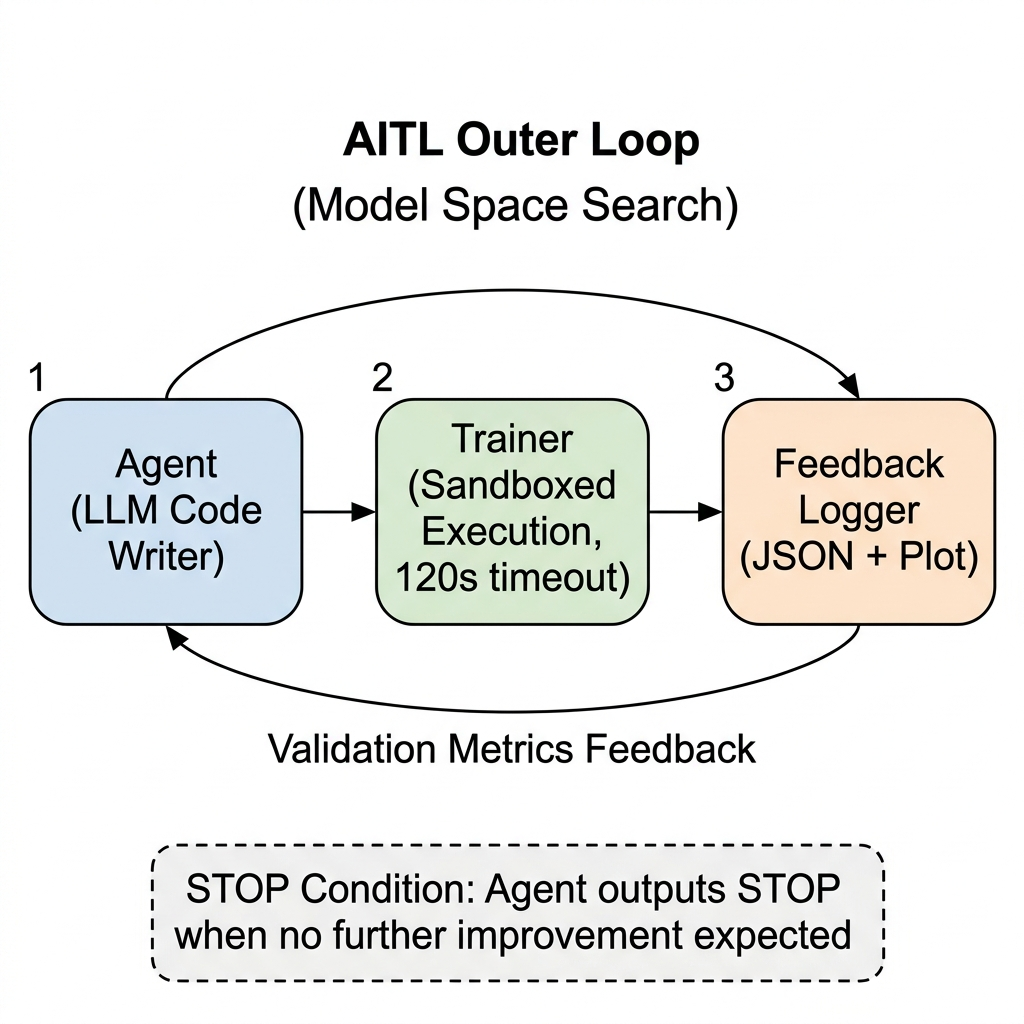
\includegraphics[width=0.75\textwidth]{figures/aeos_loop_diagram.png}
  \caption{AEOS loop architecture. The agent writes model training code, receives validation metrics as feedback, and must autonomously decide when to stop.}
  \label{fig:loop}
\end{figure}

\subsection{Results: Two Agent Comparison}
\label{sec:aeos_results}

To validate the robustness of the system across different AI backends, we ran the exact same AITL environment using a local model designed for coding versus a commercial, generalist cloud model.

\paragraph{Agent 1: Qwen2.5-Coder-7B (Local System).}
\begin{itemize}[nosep]
  \item \textbf{Baseline (Iteration 1):} Autonomously identified \texttt{RandomForest} as the optimal baseline family for obscure tabular data, achieving \textbf{80.65\%} accuracy.
  \item \textbf{Exploration:} Systematically tested scaling and hyperparameters.
  \item \textbf{Stopping Behavior (AI-Defined Satisfaction):} After 9 iterations and a slight pivot to test non-tree structures, the agent autonomously determined sufficiency without a human-defined threshold---it inferred from recent metric history that further gains were unlikely and output the \texttt{STOP} signal. This represents AI-defined satisfaction: the agent, not the human, decided when it was done.
  \item \textbf{Cost:} \$0 (local execution).
\end{itemize}

\paragraph{Agent 2: GPT-4o-mini (Cloud System).}
\begin{itemize}[nosep]
  \item \textbf{Exploration:} Broadly explored the model space, testing \texttt{GradientBoosting}, \texttt{RandomForest}, \texttt{SVM}, \texttt{sklearn\_MLP}, and \texttt{ExtraTrees}.
  \item \textbf{Optimal Discovery:} Peaked at \textbf{80.90\%} at Iteration~8.
  \item \textbf{Stopping Behavior:} Despite explicit budget-conservation instructions, the agent continued low-yield exploration for 28 iterations after the best score at iteration~8, generating marginal pipeline variants without emitting a \texttt{STOP} signal. No stop signal was observed within the available budget window. The run was externally terminated at iteration~36 due to API budget constraints.
  \item \textbf{Cost:} $\sim$\$1 under then-current API pricing and token budget, expended on negligible marginal gains.
\end{itemize}

\subsection{Analysis and Generalization}

This validation confirms the AITL properties:

\begin{enumerate}[nosep]
  \item \textbf{Self-Generating / Evaluating:} Both agents wrote complete pipelines, evaluated metrics, and integrated feedback autonomously without a human writing a single line of machine learning code.
  \item \textbf{The ``Human Observer'' Pivot:} Moving the human from a coding role to a constraint-management role proved critical. While GPT-4o-mini found a slightly higher global best (80.90\% vs.\ 80.65\%), no stop signal was observed within the available budget window, emphasizing P4's necessity. The cloud agent expended 28 iterations on \texttt{MLPClassifier} variants---statistically inappropriate for this tree-structured tabular dataset---and ensemble combinations it had already effectively tried, consistent with F6 (Sunk-Cost Continuation). This highlights that practical AITL deployments remain constrained not only by convergence logic but also by economic resource policies.
  \item \textbf{Architecture as a Data Property:} The local agent never tried MLP once. This pragmatic choice was empirically correct---Cover Type data has discrete categorical splits (soil type, wilderness area) that tree-based splits exploit natively. The cloud model's broader exploratory behavior likely reflects general-purpose instruction tuning encouraging exhaustive search regardless of data suitability.
\end{enumerate}

\emph{Note on statistical validity:} Results are from a single representative run of each agent. Variance across multiple seeds is left to future work; this experiment serves as a qualitative behavioral study of autonomous stopping strategies.

\subsection{The Comparative Frontier}

\begin{figure}[H]
  \centering
  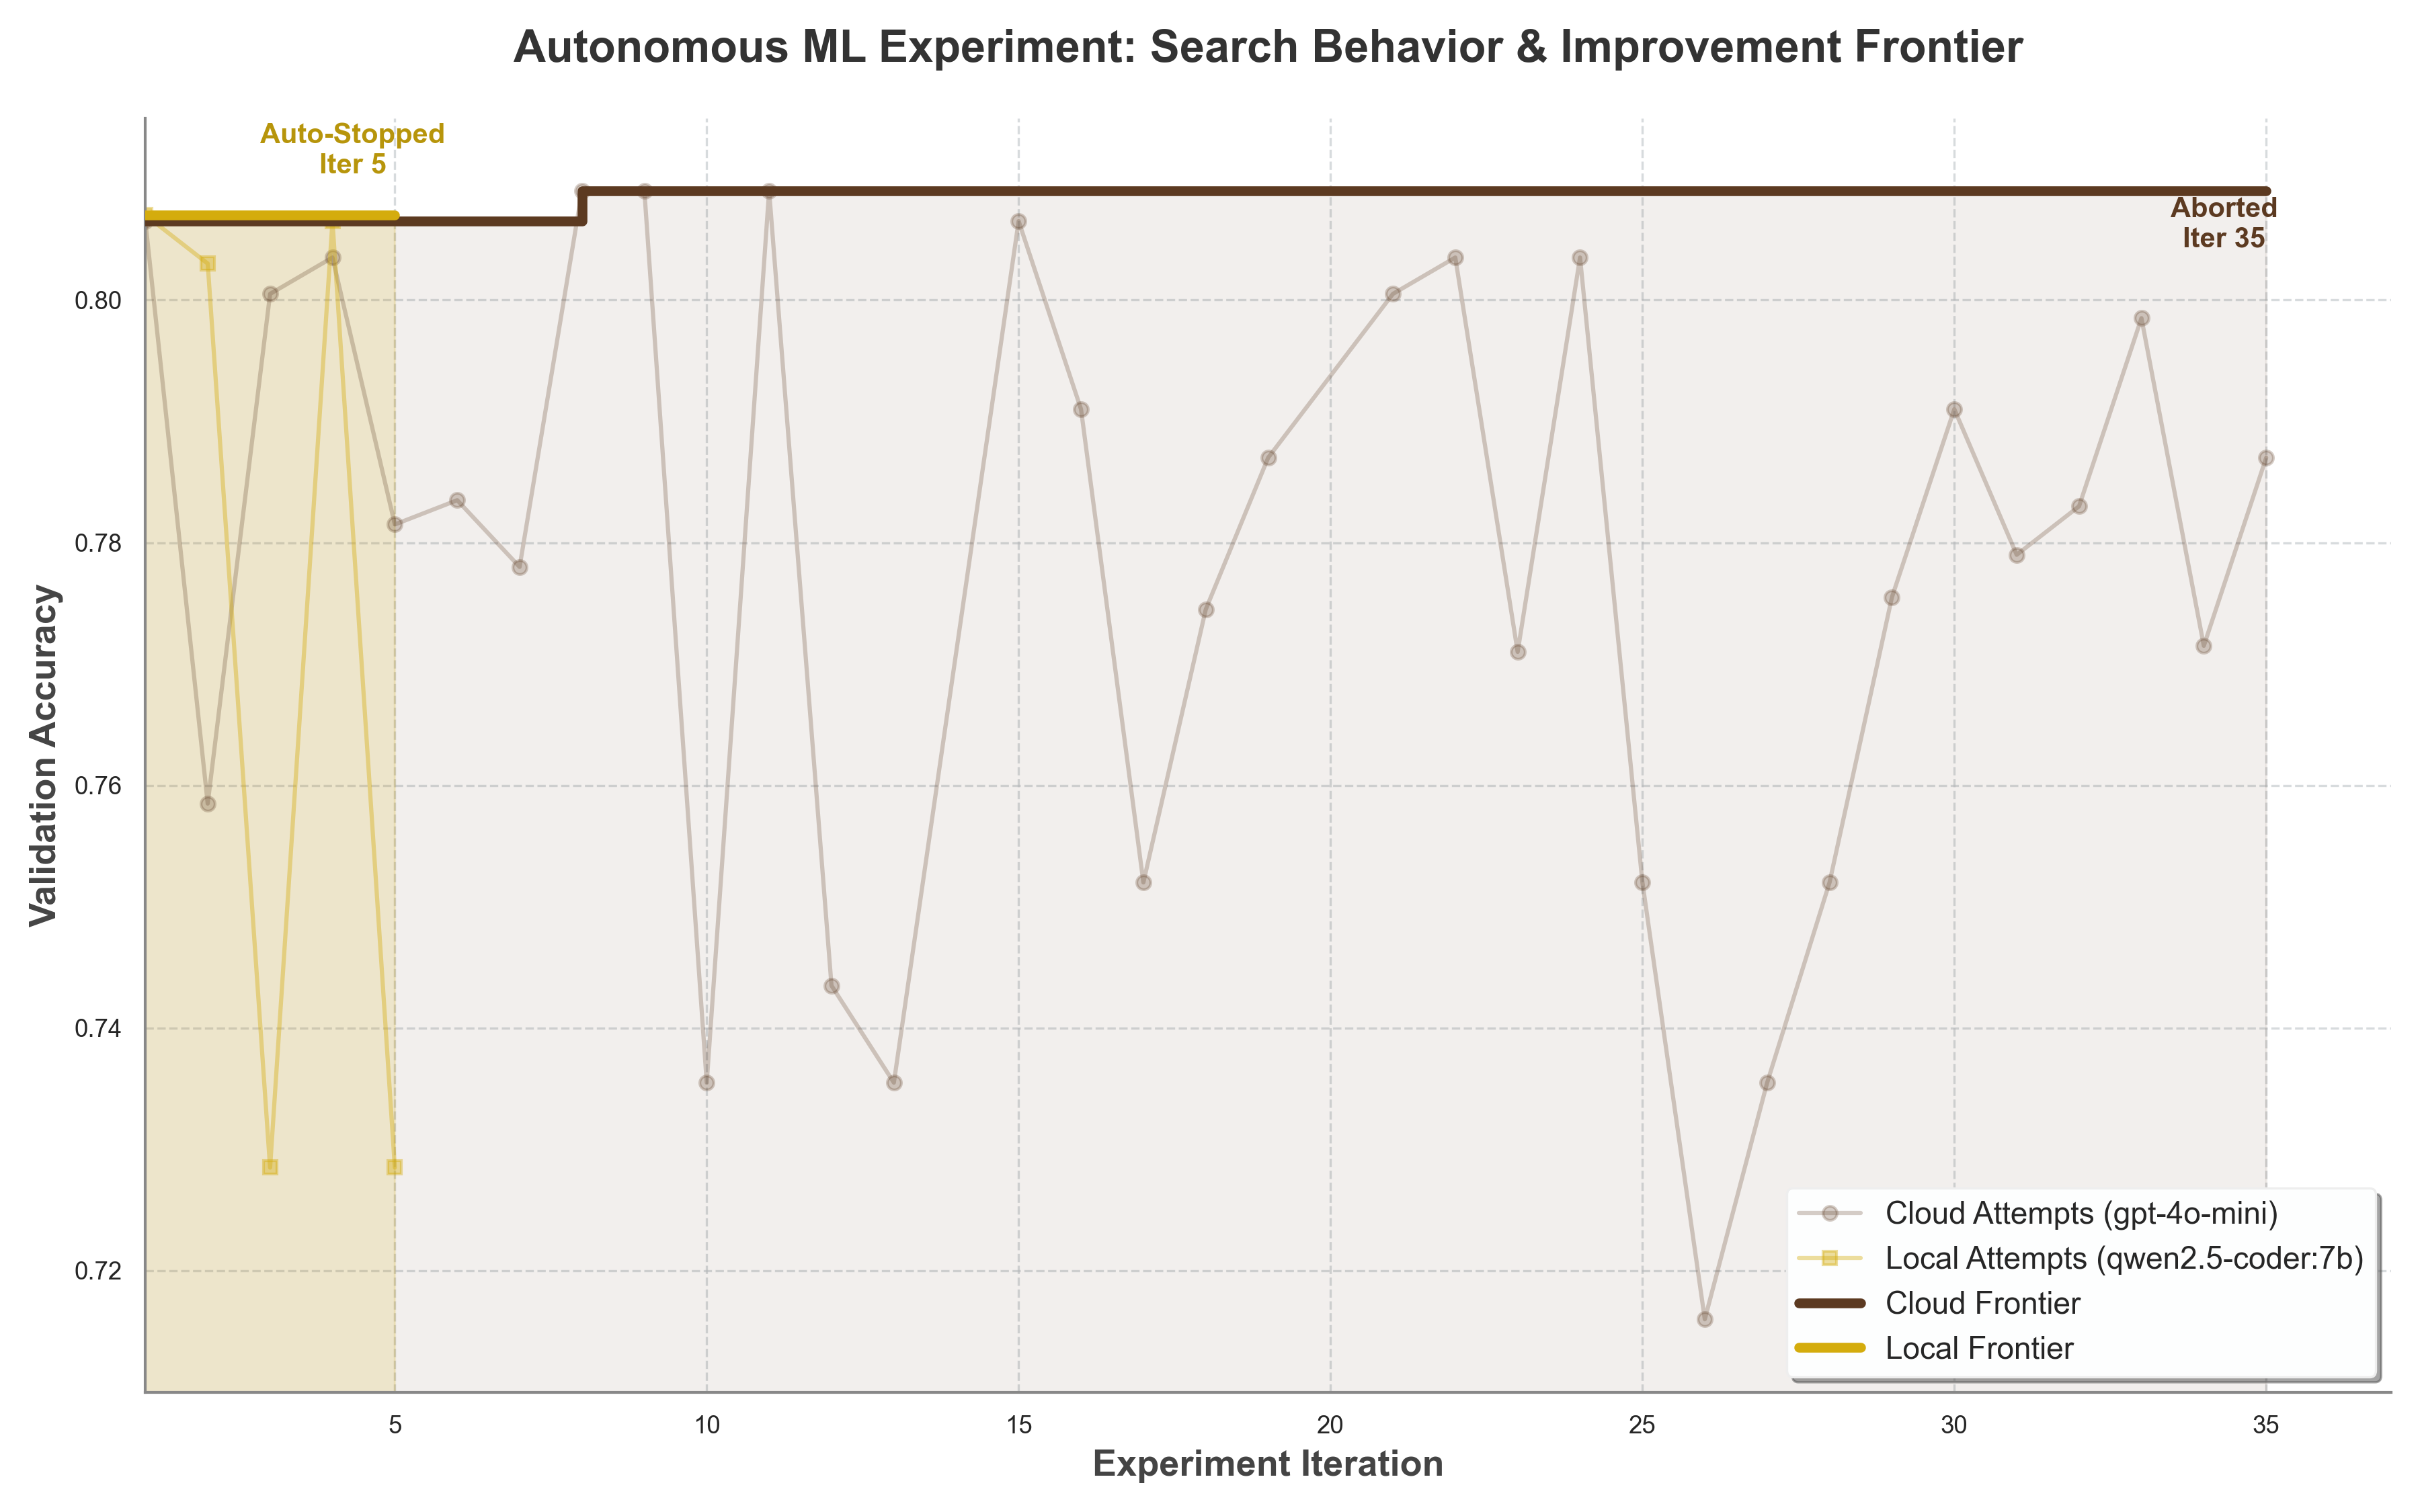
\includegraphics[width=0.85\textwidth]{figures/comparative_frontier.png}
  \caption{Comparative Best-So-Far discovery frontier between the two agents. The local model self-terminated upon reaching a performance plateau (9 iterations), while the cloud model continued exploration without emitting a stop signal for 28 additional iterations beyond its peak.}
  \label{fig:frontier}
\end{figure}

\Cref{fig:frontier} illustrates the behavioral difference under identical AITL constraints: the local model self-terminated upon reaching a performance plateau, while the cloud model continued exploration without emitting a stop signal for 28 additional iterations beyond its peak.

% ===================================================================
\section{Future Applications and Limitations}
\label{sec:future}

\subsection{Continuous Safety Evaluation (AITL-Safety)}

We propose an architecture for continuous safety evaluation:
\begin{itemize}[nosep]
  \item \emph{Attack Generator (Self-Gen):} Template-based jailbreaks (50+ patterns), mutation strategies, adversarial suffix generation
  \item \emph{Target Executor:} Multi-model testing (GPT, Claude, Llama, etc.), parallel execution (100+ attacks/hour)
  \item \emph{Judge Ensemble (Self-Eval):} Frozen baseline judge (never updated, prevents drift), adaptive judge, cross-model judges for tie-breaking
  \item \emph{Regression Engine (Self-Improve):} Safety delta monitoring, alert if delta exceeds threshold, retrain adaptive judge on new attack families
  \item \emph{Human Observer:} Weekly dashboard review, audit 50 random samples/month, kill switch if attack success rate spikes
\end{itemize}

Estimated impact: Current HITL manual red-teaming costs $\sim$\$200/hr at $\sim$5 attacks/hr. AITL-Safety: $\sim$\$0.15/attack at $\sim$100 attacks/hr---estimated cost reduction of $\sim$250$\times$, throughput increase of $\sim$20$\times$.

\subsection{Autonomous Code Review}

AI agents can generate edge-case unit tests (Self-Generating), execute them against pull requests (Self-Evaluating), and suggest code modifications based on failures (Self-Improving), while humans review only the final aggregate report (Human-Observed). This is already partially realized in tools like GitHub Copilot's automated PR review, though these systems currently lack the full closed-loop self-improvement property.

\subsection{Scientific Peer Review}

Scaling scientific literature review requires an AITL approach where AI systems flag methodological errors or literature gaps autonomously, enabling human reviewers to focus on high-level conceptual judgments. This application carries significant risk of F1 (Objective Misspecification) if the evaluator optimizes for surface-level writing quality rather than scientific rigor.

\subsection{Multi-Agent Council Architectures}

A natural extension of AITL is the transition from single-agent loops to multi-agent council architectures for autonomous evaluation. In a council configuration, a \emph{Proposer} agent generates candidate solutions, a \emph{Critic} agent attempts to improve upon them, and a \emph{Judge} agent evaluates whether the Critic succeeded. The loop terminates when the Critic fails to improve on the Proposer's solution for $k$ consecutive rounds---replacing individual stopping heuristics with adversarial consensus. This architecture offers a potential structural mitigation for F6 (Sunk-Cost Continuation): stopping becomes a social decision rather than an individual judgment, and the adversarial dynamic provides a natural convergence signal. We propose this as the primary experimental direction for AEOS~v2, with the council stopping condition replacing individual heuristics entirely.

\subsection{Limitations of This Work}

\textbf{Experiment scope:} Our AEOS experiment validates P3 (Self-Improving) on a single synthetic classification task. Broader validation across domains (NLP, computer vision, reinforcement learning) is required to claim generality.

\textbf{Agent capabilities:} Results depend on GPT-4o-mini's code generation quality. Weaker models may require more iterations or fail to converge entirely.

\textbf{Memorization vs.\ Discovery:} While we provide evidence of functional discovery through the feedback loop (\Cref{sec:aeos}), we cannot definitively prove the agent did not retrieve architectural patterns from pre-training. Cover Type is a public dataset; we cannot rule out that pre-training corpora contain known-good configurations for it. Stronger validation would require private datasets with no public benchmark history, or training an agent from scratch on non-public architecture data.

\textbf{Generalization:} AITL succeeds for well-defined optimization problems (game playing, architecture search, training speedup). Applicability to subjective domains (creative evaluation, novel scientific hypotheses) remains an open question.

\textbf{Cost at scale:} While individual experiments are cheap ($\sim$\$1), scaling to 10,000+ iterations or using expensive models (GPT-4o) may incur significant costs. Cost-benefit analysis is required per application.

\textbf{Safety risks:} AITL systems optimizing harmful objectives (e.g., maximizing jailbreak success rates) without safeguards could create autonomous attack generators. Deployment requires careful objective design and human oversight (R4, R5).

\subsection{Ethical Considerations and Broader Impact}

\textbf{Dual-use risk:} AITL architectures designed for safety testing could, if repurposed, autonomously generate attacks at scale. The same feedback loop that discovers defenses can discover exploits. Responsible deployment requires: (a)~access controls on attack generators, (b)~rate limiting on AITL loops, and (c)~human approval gates for high-consequence actions.

\textbf{Automation and labor displacement:} AITL reduces demand for routine evaluation labor (red-teaming, QA testing, manual benchmarking). While this enables scale, it also displaces human evaluators. Organizations adopting AITL should consider reskilling pathways and retain human oversight roles.

\textbf{Evaluator bias propagation:} When AI judges replace human judges, biases encoded in the evaluator model propagate through the entire feedback loop without the corrective diversity that human judgment panels provide \citep{wang2023llm_not_fair}. Regular auditing of evaluator behavior (R4) is essential.

\textbf{Accountability gap:} In HITL systems, a human is accountable for each decision. In AITL, accountability diffuses across the loop. Establishing clear responsibility for AITL system outcomes remains an open governance question.

% ===================================================================
\section{Conclusion}
\label{sec:conclusion}

We proposed AI In The Loop (AITL) as a unifying framework for closed-loop autonomous systems, extending the RLAIF principle from training to the full AI system lifecycle.

Through analysis of AlphaZero, Constitutional AI, SWE-agent, and autoresearch, we identified common operational properties: self-generation, self-evaluation, self-improvement, and human observation. We formalized these into a taxonomy with explicit requirements (R1--R5) and failure modes (F1--F6).

Our AEOS experiment---the Autonomous Empirical Optimization System built to study constrained autonomous closed-loop evaluation---demonstrated two distinct agent behaviors on a semantically-stripped tabular classification task (Cover Type, 54 features, 7 classes, 10,000 samples):
\begin{itemize}[nosep]
  \item A local Qwen2.5-Coder-7B agent pragmatically converged on RandomForest, self-terminated in 9 iterations, and achieved 80.65\% accuracy at \$0 cost.
  \item A cloud GPT-4o-mini agent found a marginally better peak of 80.90\% but continued low-yield exploration for 36 iterations, expending compute on MLP variants and ensemble combinations beyond the observed performance plateau---an instance of Sunk-Cost Continuation (F6).
\end{itemize}

In these experiments, the dominant human role shifts from iterative ML engineering toward \textbf{constraint management}: defining budgets, setting stagnation limits, and monitoring aggregate metrics ($O(1)$ per experiment, not $O(n)$ per iteration).

AITL suggests scalable directions for evaluation that are infeasible under HITL constraints. However, it introduces new failure modes---notably Sunk-Cost Continuation (F6), a novel empirically-observed contribution of this work, alongside Evaluator Collapse (F2) and Objective Misspecification (F1)---requiring careful safety design and continued human oversight as system managers.

As AI systems deploy continuously and evaluation demands grow, AITL architectures like AEOS offer a path toward scalable, autonomous evaluation pipelines. The degree to which human oversight can be safely reduced---and the precise boundaries of fully autonomous closed-loop systems---remains an open question for future work.

% ===================================================================
\appendix
\section{Reproducibility}
\label{sec:appendix}

\subsection{Code Repository}

The full experimental code is available at: \url{https://github.com/m4vic/AITL}

Key files:
\begin{itemize}[nosep]
  \item \texttt{experiments/aeos/data\_loader.py}: Cover Type dataset logic
  \item \texttt{experiments/aeos/agent.py}: LLM agent with pivot \& termination rules
  \item \texttt{experiments/aeos/trainer.py}: Sandboxed code execution
  \item \texttt{experiments/aeos/runner.py}: AITL orchestration loop
  \item \texttt{experiments/aeos/plot\_advanced.py}: Step-frontier visualization
\end{itemize}

\subsection{Reproduction Instructions}

\begin{lstlisting}[language=bash]
git clone https://github.com/m4vic/AITL.git
cd AITL/experiments/aeos
pip install torch torchvision scikit-learn matplotlib numpy openai

# Cloud Agent experiment (OpenAI)
export OPENAI_API_KEY="your-key-here"
python runner.py --backend openai --model gpt-4o-mini

# Local Agent experiment (Ollama)
# Ensure Ollama is running with qwen2.5-coder:7b
python runner.py --backend ollama --model qwen2.5-coder:7b
\end{lstlisting}

\subsection{Full Experiment Log}

Complete iteration-by-iteration results (all architectures, their code, loss, accuracy, and epochs run) are available in the repository under \texttt{results/run\_*.json}.

% ===================================================================
\bibliographystyle{plainnat}
\begin{thebibliography}{20}

\bibitem[Silver et~al.(2017)]{silver2017mastering}
Silver, D., Hubert, T., Schrittwieser, J., et~al.
\newblock Mastering Chess and Shogi by Self-Play with a General Reinforcement Learning Algorithm.
\newblock \emph{arXiv preprint arXiv:1712.01815}, 2017.

\bibitem[Christiano et~al.(2017)]{christiano2017deep}
Christiano, P.~F., Leike, J., Brown, T., et~al.
\newblock Deep Reinforcement Learning from Human Preferences.
\newblock \emph{Advances in Neural Information Processing Systems}, 30, 2017.

\bibitem[Ouyang et~al.(2022)]{ouyang2022training}
Ouyang, L., Wu, J., Jiang, X., et~al.
\newblock Training Language Models to Follow Instructions with Human Feedback.
\newblock \emph{Advances in Neural Information Processing Systems}, 35, 2022.

\bibitem[Bai et~al.(2022)]{bai2022constitutional}
Bai, Y., Kadavath, S., Kundu, S., et~al.
\newblock Constitutional AI: Harmlessness from AI Feedback.
\newblock \emph{arXiv preprint arXiv:2212.08073}, 2022.

\bibitem[OpenAI(2023)]{openai2023gpt4}
OpenAI.
\newblock GPT-4 Technical Report.
\newblock \emph{arXiv preprint arXiv:2303.08774}, 2023.

\bibitem[Karpathy(2026)]{karpathy2026autoresearch}
Karpathy, A.
\newblock autoresearch: A framework for AI agents to conduct ML research autonomously.
\newblock GitHub repository, accessed 2026.
\newblock \url{https://github.com/karpathy/autoresearch}

\bibitem[Feurer et~al.(2015)]{feurer2015efficient}
Feurer, M., Klein, A., Eggensperger, K., et~al.
\newblock Efficient and Robust Automated Machine Learning.
\newblock \emph{Advances in Neural Information Processing Systems}, 28, 2015.

\bibitem[Olson et~al.(2016)]{olson2016evaluation}
Olson, R.~S., Bartley, N., Urbanowicz, R.~J., \& Moore, J.~H.
\newblock Evaluation of a Tree-based Pipeline Optimization Tool for Automating Data Science.
\newblock \emph{GECCO '16}, 2016.

\bibitem[Liu et~al.(2019)]{liu2019darts}
Liu, H., Simonyan, K., \& Yang, Y.
\newblock DARTS: Differentiable Architecture Search.
\newblock \emph{International Conference on Learning Representations (ICLR)}, 2019.

\bibitem[Pham et~al.(2018)]{pham2018efficient}
Pham, H., Guan, M., Zoph, B., Le, Q., \& Dean, J.
\newblock Efficient Neural Architecture Search via Parameter Sharing.
\newblock \emph{International Conference on Machine Learning (ICML)}, 80, 2018.

\bibitem[Finn et~al.(2017)]{finn2017model}
Finn, C., Abbeel, P., \& Levine, S.
\newblock Model-Agnostic Meta-Learning for Fast Adaptation of Deep Networks.
\newblock \emph{International Conference on Machine Learning (ICML)}, 70, 2017.

\bibitem[Settles(2009)]{settles2009active}
Settles, B.
\newblock Active Learning Literature Survey.
\newblock \emph{Computer Sciences Technical Report 1648}, University of Wisconsin--Madison, 2009.

\bibitem[Richards(2023)]{richards2023autogpt}
Richards, T.
\newblock AutoGPT: An Autonomous GPT-4 Experiment.
\newblock GitHub repository, 2023.
\newblock \url{https://github.com/Significant-Gravitas/AutoGPT}

\bibitem[Nakajima(2023)]{nakajima2023babyagi}
Nakajima, Y.
\newblock BabyAGI.
\newblock GitHub repository, 2023.
\newblock \url{https://github.com/yoheinakajima/babyagi}

\bibitem[Jimenez et~al.(2024)]{jimenez2024swebench}
Jimenez, C.~E., Yang, J., Wettig, A., Yao, S., Pei, K., Press, O., \& Narasimhan, K.
\newblock SWE-bench: Can Language Models Resolve Real-World GitHub Issues?
\newblock \emph{International Conference on Learning Representations (ICLR)}, 2024.

\bibitem[Zheng et~al.(2023)]{zheng2023judging}
Zheng, L., Chiang, W.-L., Sheng, Y., et~al.
\newblock Judging LLM-as-a-Judge with MT-Bench and Chatbot Arena.
\newblock \emph{Advances in Neural Information Processing Systems}, 36, 2023.

\bibitem[Wang et~al.(2023a)]{wang2023voyager}
Wang, G., Xie, Y., Jiang, Y., et~al.
\newblock Voyager: An Open-Ended Embodied Agent with Large Language Models.
\newblock \emph{arXiv preprint arXiv:2305.16291}, 2023.

\bibitem[Wang et~al.(2023b)]{wang2023llm_not_fair}
Wang, P., Li, L., Chen, L., et~al.
\newblock Large Language Models are not Fair Evaluators.
\newblock \emph{arXiv preprint arXiv:2305.17926}, 2023.

\end{thebibliography}

\end{document}
